\section{Hyper Content}
	In this section we describe the algorithm we created to show synchronized interactive content to clients.


	\subsection{Content creation}

	Our system supports creating superimposed content to video, which is achieved by creating \ac{HTML} tags on top of the video  with the same size. The decision of which content must be displayed to each user is performed by our content scheduler which uses the user's current time in order to synchronize which content is shown or removed from the user interface.

	In order to create content, the user has the option to write simple movie captions without writing any code, otherwise, as mentioned before, it can write \ac{HTML}, \ac{CSS} and \emph{JavaScript}. The definition of the content's starting and ending time by the user it is not an easy task. 
	Figure \ref{fig:creation} shows the user interface for creating interactive hyper content manually.

	\begin{figure}[H]
		\centering
		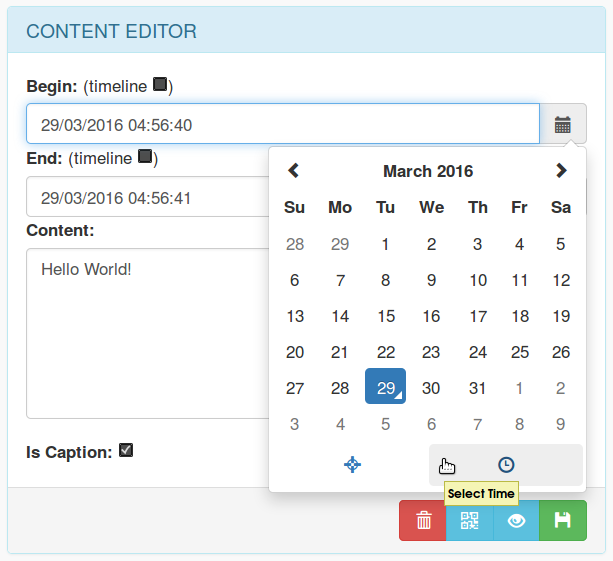
\includegraphics[width=0.5\textwidth]{figures/edition.png}
		\caption{Manual content creation}
		\label{fig:creation}
	\end{figure}

	Listing \ref{lst:createcontent} shows the structure of the content created by one user%. and Listing \ref{lst:receivecontent} shows the format of messages that users receive in order to supply their content schedulers with fresh data.

\begin{minipage}{\linewidth}
\begin{lstlisting}[caption={Example of content created by one user},label={lst:createcontent},language=json]
{
	"cmd":"createContent",
	"start":"2016-03-29T03:56:40.000Z",
	"end":"2016-03-29T03:56:41.000Z",
	"content":"<h1>Hello</h1>"
}
\end{lstlisting}
\end{minipage}


	Defining the content's time to appear in real-time would require a previous user plan. Otherwise the user could make a speech and insert the content later.


	As manually content insertion is a laborious task that can be realized after the video is recorder, we provide an alternative mechanism for real time introduction of superimposed content.	In order to help the content creator to introduce and synchronize its content in real-time, we allow the user to encode its content into \ac{QR} codes and show it to the camera in real time.

	\ac{KMS} lets registering event handlers for \ac{QR} code detection. The component that detects \ac{QR} codes on \ac{KMS} is called periodically and fires the handlers with the decoded content. This mechanism does not detect if the \ac{QR} code enters or leaves the screen. We had to implement our own mechanism for detecting those events. Each user session in the server maintains a map with the contents that are present on the screen. In order to apply our algorithm more efficiently we calculate the content's hash through the \emph{md5} method. If the hash is not present in the map, it means the \ac{QR} code was entering the screen, we add that hash to the map and associate the current time to it, all the users are notified to watch that content in real-time. If the same \ac{QR} code is not detected after a time bigger then two periods we can conclude that the \ac{QR} code left the screen and we add the correspondent content into our database. Listing \ref{lst:pseudo_qrcode} shows the pseudo code for \ac{QR} code leaving detection.

\begin{minipage}{\linewidth}
\begin{lstlisting}[caption={Pseudo code for QR code leaving detection},label={lst:pseudo_qrcode},language=JavaScript]
var ongoingCodesMap = {};
var startedCodesMap = {}
function onCodeFound(content) {
	var startingTime = getCurrentTime() - getUserOffset();
	var hash = md5(content);
	if(startedCodesMap[hash] == null) {
		sendQRCodeToEditingUser(hash,content); // insert UI
		startedCodesMap[hash] = currentTime;
	}
	ongoingCodesMap[hash] = currentTime;
	waitTwoSeconds(); // onCodeFound() may be called from other threads
	var newestTime = ongoingCodesMap[hash]; 
	if(newestTime == currentTime){
		var startingTime = startedCodesMap[hash];
		var endingTime = getCurrentTime() - getUserOffset();
		startedCodesMap[hash] = null; 
		ongoingCodesMap[hash] = null; 
		sendQRCodeToEditingUser(hash,null); // remove from UI
		insertContentIntoDatabase(startingTime,endingTime,content);
		sendContentToUsers(startingTime,endingTime,content);
	}
}
\end{lstlisting}
\end{minipage}


	Our main content synchronization mechanism is time based but, with some programming knowledge, it is possible to insert \emph{JavaScript} code that fires events on user interaction. For example, after a teacher's lecture, it is possible to show a quiz to the users in order to understand what they learned and then submit the data to the server for further analysis.


	\subsection{Interactive media synchronization}

	In order to allow users to visualize past and present communications, we express the user's position as the time offset between its navigated time and the current time.


	In our solution, content is represented as simple text that can contain \ac{HTML}, \ac{CSS} or even \emph{JavaScript}. This content is displayed on defined intervals of time. Multiple contents can be displayed at the same time. In order to achieve that, we define layers above the video with the same size. Each layer is associated to the content.	We have taken into account that the amount of content tends to grow with time and the user should only have access to a subset of the content instead of all of it, which would be very inefficient. The content to display for each user depends on the user's position on the time-line. This position is given by an offset between the current time and the navigated time. If the user is watching the content in real-time this offset is always zero. If the user is reproducing past communications in normal playback rate, this offset is constant and, as a consequence, there is need to re-synchronize this value. If, for instance, we had to implement communication reproduction with a faster or slower playback rate, we would need to take into account the fact of this time offset not being constant. 

	Each content is divided into two components, the \emph{start} and the \emph{end} which are sent to users. The \emph{start} component contains a time stamp, the content identification number and the content itself in form of text. The \emph{end} component only contains the time stamp and the content identification number. 

	The users will receive their contents from the server on five different situations:

	\begin{itemize}
		\item Conference room entrance (advertised by server).
		\item Set of events empty and server has more content (client requested).
		\item Content is created (advertised by server).
		\item Content is removed (advertised by server).
		\item User navigates to different point in time (client requested).
	\end{itemize}

	The content to return is given by the union of the two following content subsets:
	\begin{itemize}
		\item Content that should be currently on display.
		\item A subset of contents whose starting time is immediately following the user's time.
	\end{itemize}

	The second subset is used for predicting which content the user will watch and avoid requests during its events.

	The content description messages that are sent to each user contains the constant itself on the form of a list of events and an attribute that specifies if the server has more content to return.

	Listing \ref{lst:sentcontent} shows the structure of the content sent to users.

\begin{minipage}{\linewidth}
\begin{lstlisting}[caption={Exampe of content sent to users},label={lst:sentcontent},language=json]
{
	"cmd":"content",
	"data":[
		{
			"id":"56f9fd1aa986c615fab43d69",
			"time":"2016-03-29T03:56:40.000Z",
			"type":"start",
			"content":"<h1>Hello</h1>"
		},
		{
			"id":"56f9fd1aa986c615fab43d69",
			"time":"2016-03-29T03:56:41.000Z",
			"type":"end"
		}
	],
	"more":false
}
\end{lstlisting}
\end{minipage}

	When a user enters the conference room, immediately after the \emph{WebSocket} creation the server sends him the current content. The user receives the content, sorts all components by time and creates a set of events. All the events before the user's time are displayed and removed from the set of events. A timer is scheduled for the first component on the event set and the process repeats while the set is not empty.

	If the event set is empty, there two options. If the server contained more content, a new request for content is made and the process starts from the beginning, namely the server sends the correspondent content again. If the server has no more content, the process is stopped until it sends more.

	Listing \ref{lst:pseudo_render} presents the pseudo code for our content scheduler.

\begin{minipage}{\linewidth}
\begin{lstlisting}[caption={Pseudo code for hyper content scheduler},label={lst:pseudo_render},language=JavaScript]
function scheduleContent() {
    var navigatedTime = getCurrentTime() - getUserOffset();
    while ( hasLocalEvents() ) {
        if ( firstEventIsOlderThan(navigatedTime)) {
            if ( firstEventIsStart() ) {
            	addHtmlLayer(event);
            } else {
            	removeHtmlLayer(event);
            }
            removeFirstEvent();
        } else {
            break;
        }
    }
    if ( hasNoLocalEvents() && serverHadNoMoreContent()) {
    	return;	// nothing to do
    } 
    if ( hasNoStartEvents() && serverHadMoreContent() ) { 
       	requestContentFromServer(navigatedTime);
    } else {
        waitUntilNextEvent();
        scheduleContent();
    }
}
\end{lstlisting}
\end{minipage}

	\subsection{Content Removal}
		Each layer is identified by its content identification number which is used by our content scheduler in order to remove disappearing content.

		If a user clicks over one layer's content the layer becomes selected (a frame is drawn around it) and its content identification number is added to a list containing the selected layers. When a user wishes to remove superimposed content, the selected layer ids are sent to the application server, with the same format as shown on Listing \ref{lst:deletecontent}, and subsequently all users will receive a message in order to update their user interface.


\begin{minipage}{\linewidth}
\begin{lstlisting}[caption={Example of removing content message sent by one user},label={lst:deletecontent},language=json]
{
	"cmd":"deleteContent",
	"content":["56f9fd1aa986c615fab43d69","57339588ac687b423e5b3a1e"]
}
\end{lstlisting}
\end{minipage}

	\subsection{Security Concerns}

	Our solution is flexible on what kind of interactions are possible to the users in real time, but allowing users to write \emph{JavaScript} that is executed on the other users browser would attackers to misuse their resources and access critical information. We could solve this problem easily by escaping any \emph{script} tag present on the content, but we would sacrifice the kind of interactions that are possible. By not allowing \emph{JavaScript} we would need to implement a subset of conceivable actions a priori and fire them when a type of message is received. We decided to ignore the security vulnerabilities that are exposed by evaluating \emph{JavaScript} because, in order to offer the same interactions, we would have to do an exhaustive functional requirements gathering and, in our prototype, our goal is to explore users behavior when interacting with our system. 

	Another way to solve this problem, which is not within the goals of this thesis, is to analyze the \emph{JavaScript} code and detect if it is malicious. Although we have not performed a detailed study on this field, we are aware of its complexity and the existence of solutions to deal with this problem, in particular \emph{EarlyBird}\cite{earlybird} came to our attention. 

\emph{EarlyBird} uses machine learning techniques in order to improve malicious \emph{JavaScript} code detection accuracy.


	\subsection{Time Manipulation}

	We have used \emph{vis.js} to display out time-line. This library was created for content navigation through time, but it was not designed to be always moving automatically. We have created a background timer that performs the animation of moving the window of time bounds and user navigated time marker.

	Figure \ref{fig:timeline} shows the graphical appearance of our interactive time-line. In order to navigate through time, the user must drag and drop the time-line horizontally. When the user drops the time-line an event handler is called with the new user's time offset, which will be used to send a message to the server in order to choose the correspondent content to display. 

	\begin{figure}
		\centering
		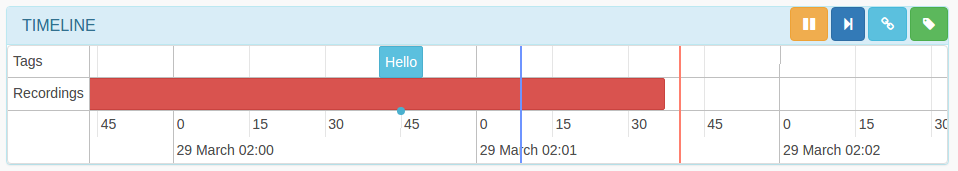
\includegraphics[width=0.95\textwidth]{figures/timeline.png}
		\caption{Interactive time-line}
		\label{fig:timeline}
	\end{figure}

	We have noticed the server time being different from client time and this created timing inconsistencies, such as showing existing recorded blocks of movie in the future. To solve this problem, the server sends its time to the client immediately after the \emph{webSocket} creation. We synchronize the time-line with the server and although it may exist a small error due to network transmission time, the graphical error is negligible. 


	\subsection{Time annotations creation}

	Time annotations are a simpler way to mark points in time and share them with other users. When a user enters a conference room, the server sends all annotations so they can be displayed directly into the user time-line. When each time annotation is created, all users are notified so they can update their interfaces.

	Figure \ref{fig:annotation} shows the creation and placement of annotations on the time-line. To save the annotation the user must click on the floppy icon in order to save it and notify the conference participants. 

	\begin{figure}
		\centering
		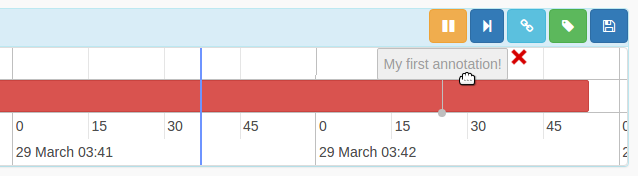
\includegraphics[width=0.7\textwidth]{figures/annotation.png}
		\caption{Creating a time annotation}
		\label{fig:annotation}
	\end{figure}

	Besides the ability to create tags, it is also possible to create time hyper-links, see Figure \ref{fig:timelink}, that can be sent to other users externally so they can navigate directly to the content when entering the conference room.


	\begin{figure}
		\centering
		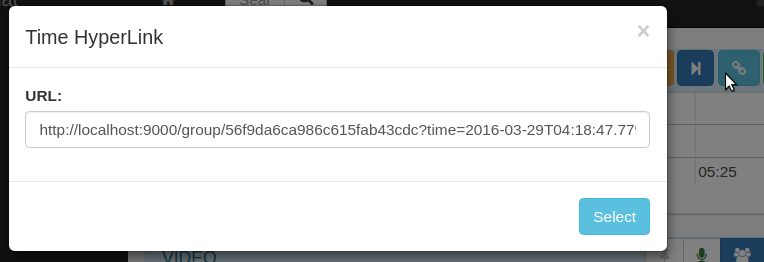
\includegraphics[width=0.8\textwidth]{figures/timelink.png}
		\caption{Time link creation}
		\label{fig:timelink}
	\end{figure}


	\subsection{Content Search}

	Users can search for annotations and contents and travel to their correspondent times. In the case of hyper content, after handling the result from database, we extract the text by discarding \ac{HTML} tags with \emph{Jsoup}\footnote{\url{http://jsoup.org/} (Accessed 21 March 2016)} and apply the query again. We extract the text from \ac{HTML} because accidentally searching for text contained in \ac{HTML} tags would lead to incorrect results.

	Figure \ref{fig:search} shows how the search results are displayed to the user. Each result entry contains an icon specifying the type of result (hyper content, time annotation, ...).




\begin{figure}
	\centering
	\begin{minipage}[b]{0.55\linewidth}
		\centering
		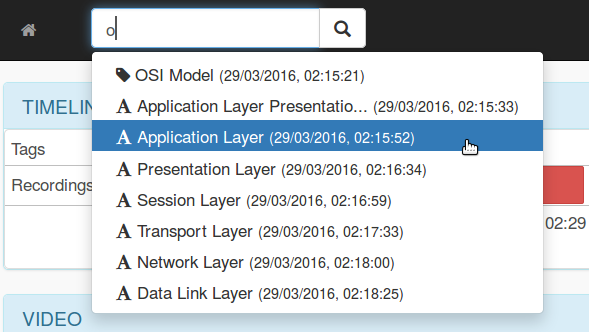
\includegraphics[width=\textwidth]{figures/search.png}
		a) Result list
	\end{minipage}
	\quad
	\begin{minipage}[b]{0.40\linewidth}
		\centering
		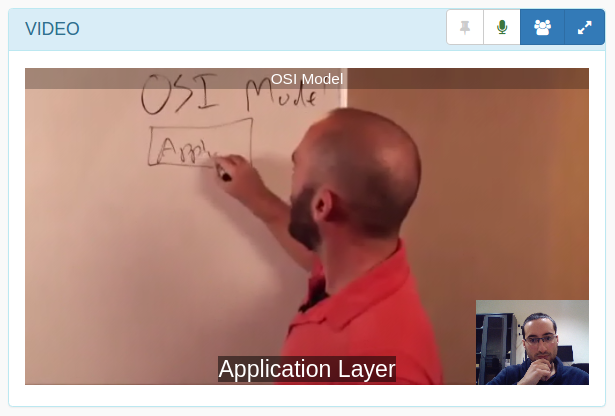
\includegraphics[width=\textwidth]{figures/search2.png}
	    b) Selected result
	\end{minipage}
	\caption{Example of search results}
	\label{fig:search}
\end{figure}


	\subsection{View composition and switching view}

		In order to show all streams to all users, each conference participant could receive individual streams for each user that share video. In overall, if there were $n$ active participants in the conference room, the number of streams per user would be $n$ ($1$ for sending video and $n-1$ for receiving) and, consequently, the number of streams in that conference room, as observed in Figure \ref{fig:xcomposite}, would be $n^2$.


\begin{figure}
\centering
\begin{minipage}[b]{0.45\linewidth}
	\centering
	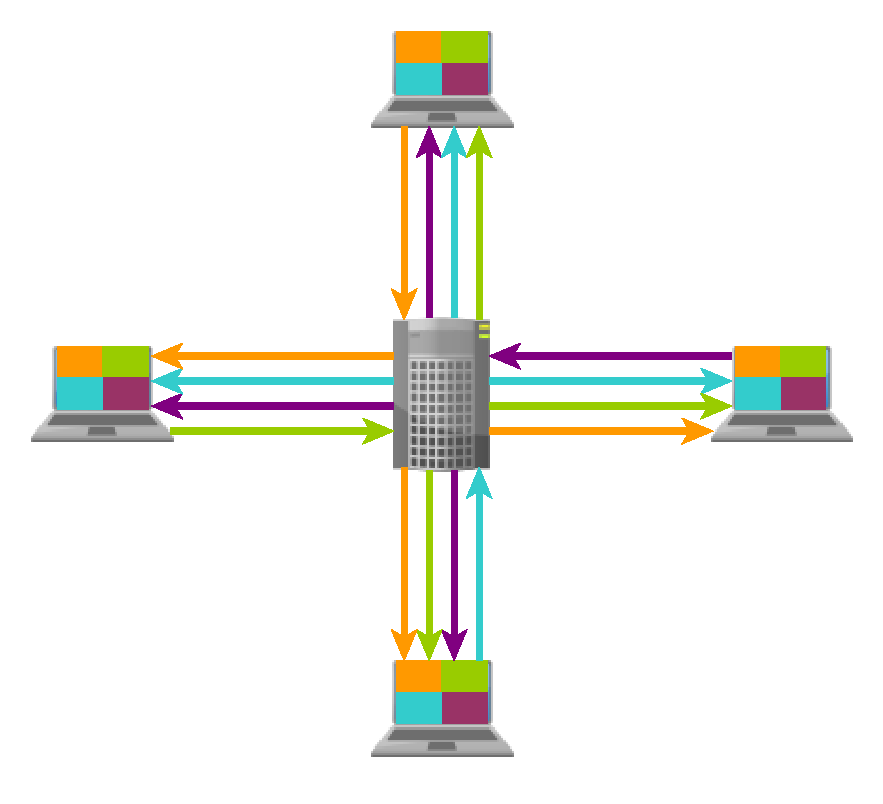
\includegraphics[width=\textwidth]{figures/xcomposite.pdf}
		\caption{Client-side stream composition}
	\label{fig:xcomposite}
\end{minipage}
\quad
\begin{minipage}[b]{0.45\linewidth}
	\centering
	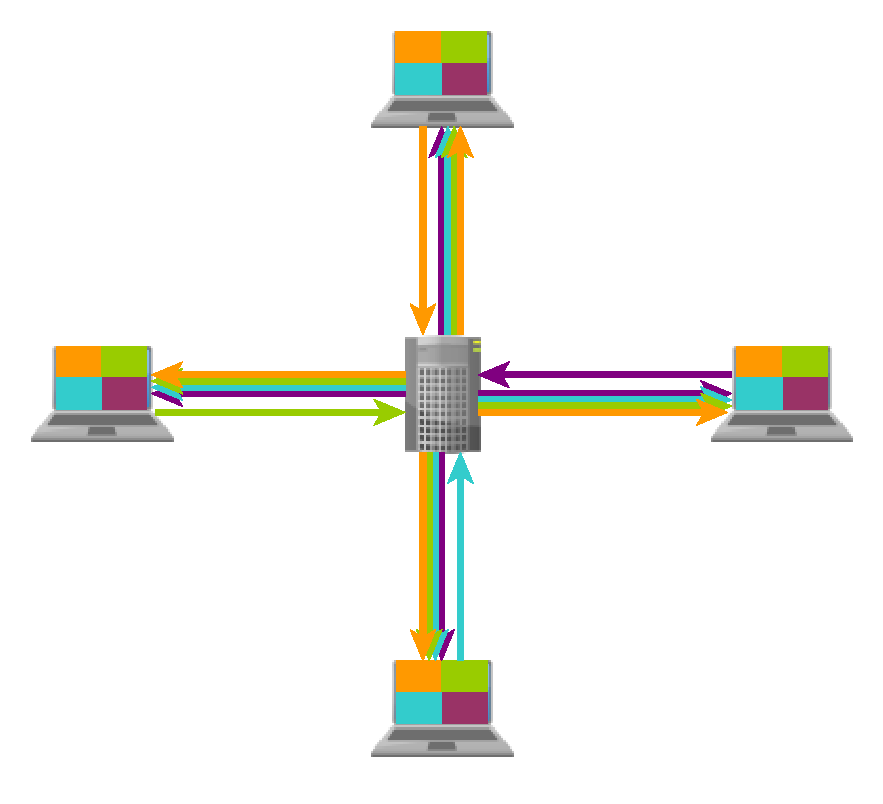
\includegraphics[width=\textwidth]{figures/ecomposite.pdf}
		\caption{Server-side stream composition}
	\label{fig:ecomposite}
\end{minipage}
\end{figure}


		By mixing all streams into a single one, users can receive a single stream with the representation of all active users. With this approach, the total number of streams within a conference room can be, at most, $2n$ (each user has $2$ streams, one to send and another to receive) as observed in Figure \ref{fig:ecomposite}.

		The numbers we have presented above were calculated taking into account that all users would receive and send video at the same time, which is the worst case scenario, although users may choose just receiving streams.

		When the amount of participants is just two, both solutions require the same amount of streams but as the number of participants increase, the composition operation tends to be a more efficient approach. 

		The composite operation, as shown on figure \ref{fig:wcomposite}, is performed at \ac{KMS} and works by decoding the incoming client streams, mixing audio and video and encoding again to send back to users.

	\begin{figure}
		\centering
		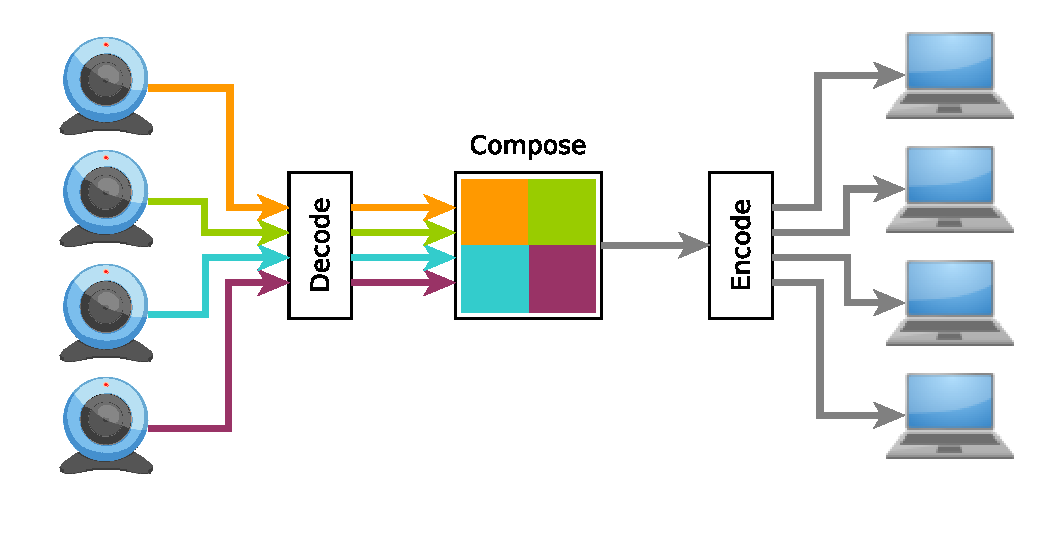
\includegraphics[width=0.7\textwidth]{figures/wcomposite.pdf}
		\caption{Stream decoding, composition and encoding}
		\label{fig:wcomposite}
	\end{figure}


		We provide a way for users to select the composite view of the conference room or the video shared by a particular user device as it can be seen on figure \ref{fig:devices}. 
	
	\begin{figure}
		\centering
		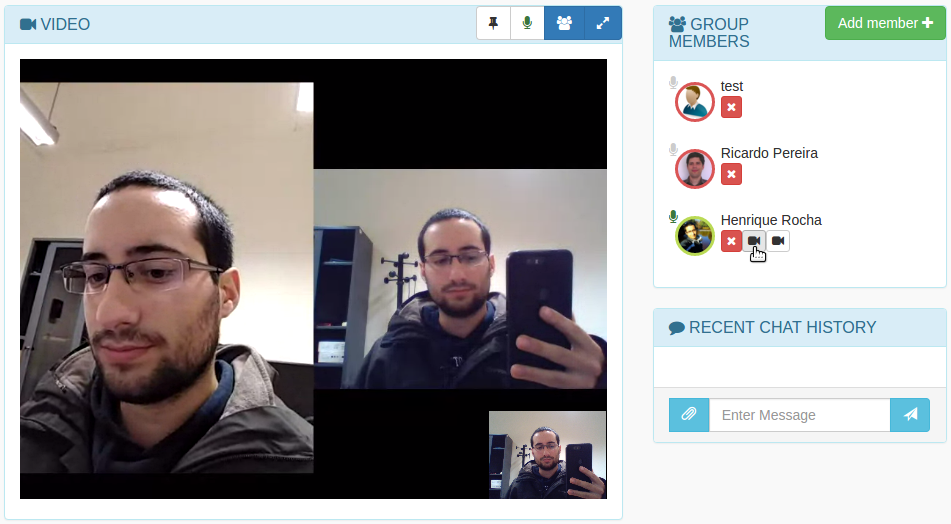
\includegraphics[width=0.7\textwidth]{figures/devices.png}
		\caption{Multiple devices per user}
		\label{fig:devices}
	\end{figure}


		When a user plays or ends playing a block of recorded video, it requests a list of available devices from each user that can be played at the navigated time by querying the database.

		On the other hand, if a user changes to real time, the list of devices is extracted from the set of \emph{webSockets} that are associated to the respective conference room. This list of devices is also sent to the users that are also in real time mode whenever a new user enters or leaves the conference room.

		In addition to select a stream to view, which remains the same if not interrupted, we also provide an automatic mechanism for switching the view to the current speaker. With respect to sound analysis, the sound samples are analyzed on the client side through the web audio \ac{API}.

		Our speech detector is straightforward, we could perform a spectral analysis in order to understand if the analyzed sound contains frequencies in the range of the human voice but instead we just capture sound samples in real time and calculate the maximum sound amplitude. If a sound sample has an amplitude bigger than a factor of the maximum amplitude (we have used an empirical value of 10\%) we say that the user is speaking and therefore we send a message to the server if the speaking state has changed. Subsequently, the server receives the user speaking state and sends it to the other users so they can request a different view.

		If multiple participants are talking at the same time, the selected view will change indeterminately between them. Although such behavior is not the most desired, we could have done a dedicated composite view in order to show the talking participants. 

\subsection{Non interactive media synchronization}
		By default, each user receives the real time mixed video and audio of every users. As described on the previous section, users can switch the current view even for recorded media.

		Whenever a user changes the current viewed time, our server calculates which chunks to reproduce.In order to determine which chunks are going to be played we could find any chunk that matches the session id and intersects the given user time. Although this seems logical, we limit the size of the results to one and ignore the starting component of the recording chunk. As a consequence, we will obtain the recording chunk that ends right after the playing time.

		The obtained chunk may or not intersect the given time. If it intersects then we immediately start playing the chunk, otherwise we know that the chunks starting time is after the playing time and we schedule the player to reproduce after a time duration given by the difference of the playing time and chunk starting time.

		In order to reduce the delay between switching parts we perform a query on the database for finding the next chunk to play while the selected media is still playing. In order to find the next chunk, we use the chunk that has a bigger id immediately after the playing chunk.

		In order to allow the users to watch an individual image and ear the audio of everyone, we are using two players, one for audio and another for video. 

		If a user leaves a conference room, it is expected that the sequence of played blocks ends. When a block is not found for a given \emph{webSocket} session, we try to find a block for the same user and if not possible, we try to play a composite recorded block, lastly, if every attempt fails we wait for the next interval that contains media.

\subsection{Chat}
		Not less important the chat functionality was implemented using \emph{webSockets}. When a message is sent by a user, it is received by the server, which records it and sends to all the users.

		In order to support receiving a huge amount of messages and not having a bottleneck when loading the conference room, we just load an amount of messages that fill the chat panel. When a user scrolls the chat to read old messages, we detect when the chat scroll bar reaches the limit and request older messages from the server automatically.

		Moreover, when the clients receive messages, whether older or newer ones, their ids are used to place them in the correct position. In other words, older messages are placed in the top of the chat panel and newer ones in the bottom.

		Besides that, we also support sending files to other users, which are stored on the database and accessed through an \ac{URL}.

\subsection{Collaborative editor}

Our collaborative editor is a simple text editor that is synchronized with all participants within a conference room implemented using \emph{ot.js}.

The state of our collaborative editor is not saved on the database every time it changes. Instead, the users just synchronize the editor content among themselves using the application server to relay editor changes and save on demand.

When a user joins a conference room and the content differs from the version stored in the database, our server does not have the right content to deliver the user. As a consequence, our server names a random participant to yield its collaborative content and delivers it to the joining user.

All operations that we perform over the conference room's collaborative editor are performed in mutual exclusion so all updates are delivered in the same order to all participants. For example consider two write events $W_1$ and $W_2$ if they occur at the same time, our server will receive one of the events first, say $W_1$, and delivers is to every users including its writer. Only then the server delivers the $W_2$ content. With this serialization mechanism we can ensure the content is equal on every user editor.

According to \emph{ot.js} there are three types of operations:
\begin{itemize}
\item{retain} $\rightarrow$ advance the cursor by a given number of positions.
\item{insert} $\rightarrow$ write the given text in the current position.
\item{delete} $\rightarrow$ delete a given number of characters forward.
\end{itemize}

In summary, our server just ensures the ordering of operations and delivers the messages among users without even parsing the message's content.